\chapter{Banana Pi}

Banana Pi ist eine Reihe von Minicomputern, die hauptsächlich zur Entwicklung in Hobbyprojekten, Home-Automation und zu Lehrzwecken in Schulen und Universitäten eingesetzt werden.
Sämtliche verfügbare Modelle sind Ein-Platinen-Computer, die darauf ausgelegt sind, möglichst günstig produziert werden zu können. Das Design und der Nutzengedanke hinter der 
Banana Pi-Serie wurde stark von den Raspberry Pi-Minicomputern beeinflusst, die eine ähnliche Größe, Verwendung und Kosten aufweisen.
\\[1ex]
Neben dem bekanntesten Modell \textit{Banana Pi M1} (s. \autoref{pic:bpim1}) und seinen verbesserten Versionen M1+, M2, M2+, M2 Ultra und M3, gibt es weitere, spezialisierte Versionen:
\begin{itemize}
	\item Banana Pi M64, für 64-Bit Betriebssysteme
	\item Banana Pi G1, für \ac{IoT}-Entwicklung mit WLAN, ZigBee und Bluetooth (s. \autoref{pic:bpig1})
	\item Banana Pi D1, mit eingebauter Kamera (s. \autoref{pic:bpid1})
	\item Banana Pi R1, mit vier zusätzlichen Ethernet-Ports (s. \autoref{pic:bpir1})
\end{itemize}
\begin{figure}[!htbp]
\caption{Banana Pi M1}
\source{https://upload.wikimedia.org/wikipedia/commons/6/63/BPI-M1.jpg}
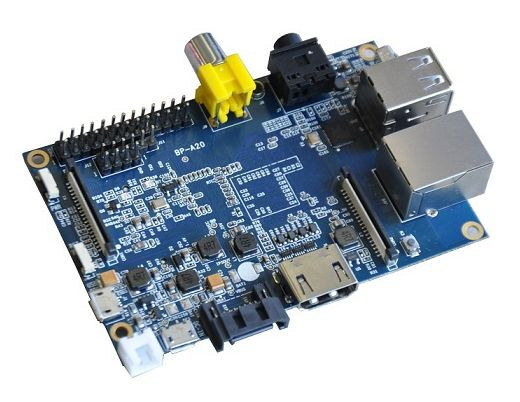
\includegraphics[width=0.5\textwidth]{content/pictures/bpim1.jpg}
\label{pic:bpim1}
\end{figure}
\begin{figure}[!htbp]
\caption{Banana Pi G1}
\source{http://www.banana-pi.com/tp/2015013018534129497.JPG}
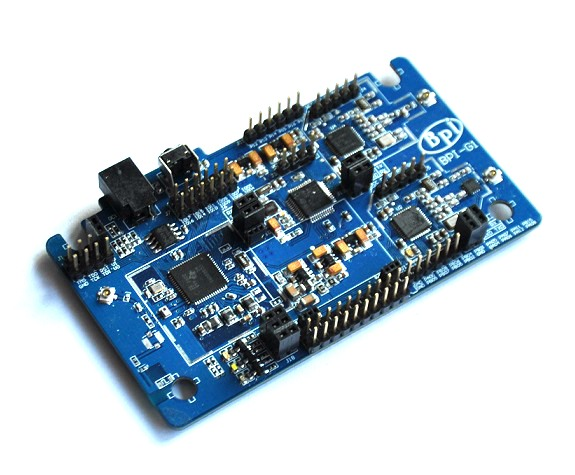
\includegraphics[width=0.5\textwidth]{content/pictures/bpig1.jpg}
\label{pic:bpig1}
\end{figure}
\begin{figure}[!htbp]
\caption{Banana Pi D1}
\source{https://upload.wikimedia.org/wikipedia/commons/c/c7/BananaPi-D1.jpg}
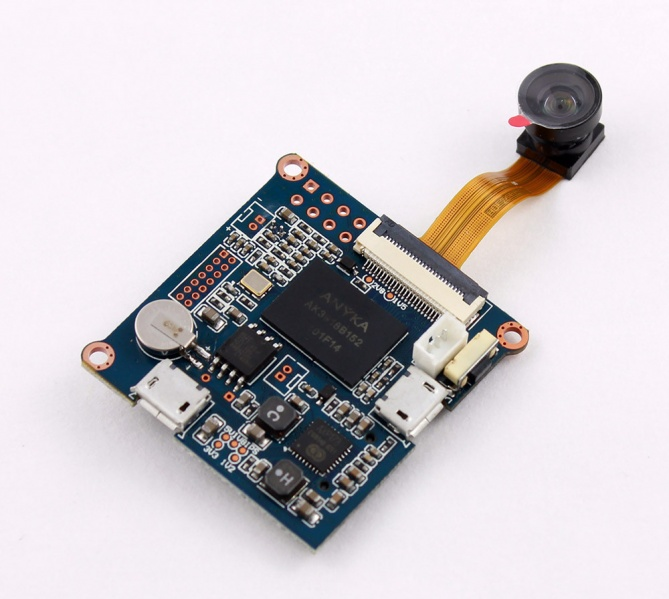
\includegraphics[width=0.5\textwidth]{content/pictures/bpid1.jpg}
\label{pic:bpid1}
\end{figure}
\begin{figure}[!htbp]
\caption{Banana Pi R1}
\source{http://www.banana-pi.com/tp/2014082202191761603.JPG}
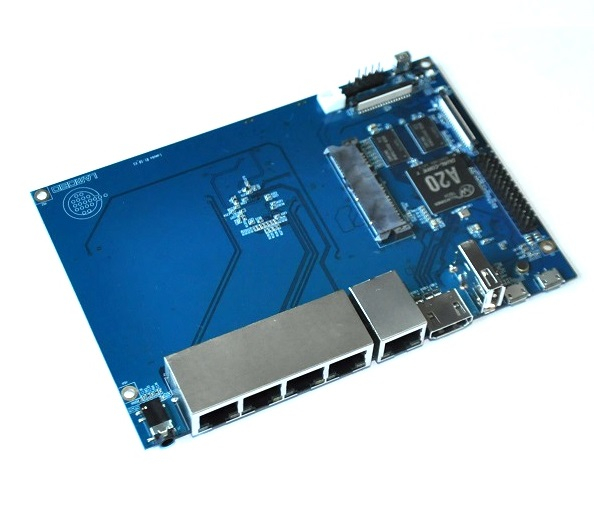
\includegraphics[width=0.5\textwidth]{content/pictures/bpir1.jpg}
\label{pic:bpir1}
\end{figure}

\section{Hersteller}


\section{Banana Pi R1}


\section{Informationsquellen}
